\documentclass[tikz,border=5pt]{standalone}
\usepackage{luatexja}
\usepackage[hiragino-pron]{luatexja-preset}
\usepackage{amsmath,amssymb}
\usetikzlibrary{matrix,fit,positioning}

\begin{document}
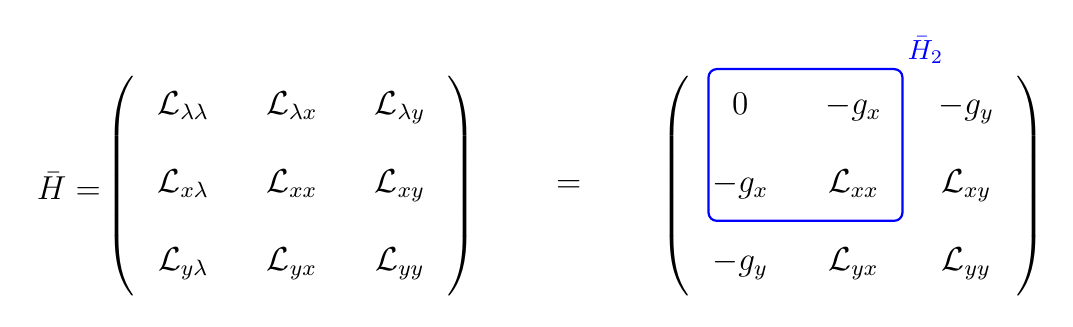
\begin{tikzpicture}[every node/.style={font=\large}]

% First matrix (L-subscript form)
\matrix[matrix of math nodes, left delimiter=(, right delimiter=),
  row sep=10pt, column sep=14pt] (A) {
  \mathcal{L}_{\lambda\lambda} & \mathcal{L}_{\lambda x} & \mathcal{L}_{\lambda y} \\
  \mathcal{L}_{x\lambda} & \mathcal{L}_{xx} & \mathcal{L}_{xy} \\
  \mathcal{L}_{y\lambda} & \mathcal{L}_{yx} & \mathcal{L}_{yy} \\
};

\node[left=10pt] at (A.west) {$\bar{H} =$};

% Second matrix (explicit form)
\matrix[matrix of math nodes, left delimiter=(, right delimiter=),
  row sep=10pt, column sep=14pt, anchor=west] (B) at ([xshift=90pt]A.east) {
  0 & -g_x & -g_y \\
  -g_x & \mathcal{L}_{xx} & \mathcal{L}_{xy} \\
  -g_y & \mathcal{L}_{yx} & \mathcal{L}_{yy} \\
};

% Equals sign between the two matrices
\node at ([xshift=45pt]A.east) {$=$};

% H_2 box (top-left 2x2)
\node[draw=blue, thick, rounded corners=3pt,
  fit=(B-1-1)(B-2-2), inner sep=5pt] (box) {};
\node[blue, font=\normalsize] at (box.north east) [above right=-2pt and -2pt] {$\bar{H}_2$};

\end{tikzpicture}
\end{document}
